\documentclass[10pt, a4paper]{article}

\usepackage{ctex}
\usepackage{xeCJK}
\usepackage{caption}
\usepackage{geometry}
\geometry{
    left = 0.6in,
    right = 0.6in,
    top = 0.8in,
    bottom = 1.0in
}
\usepackage{amssymb}
\usepackage{amsbsy}
\usepackage{amsmath}
\usepackage{xcolor}
\usepackage{mathrsfs}
\usepackage{graphicx}
\usepackage{pifont}
\usepackage{tasks}
\settasks{
    label = \Alph*. ,
    label-width = 16pt
}
\pagestyle{empty}

\newcommand{\Title}[3]{
    \begin{center}
        \Large \textbf{中国电子学会 #1~年~#2~月 Scratch~#3级考试}
    \end{center}
}
\newcommand{\TimeAndName}[1]{
    \begin{center}
        考试时间:~#1~ 分钟 \qquad\qquad\qquad\qquad 姓名:\underline{\quad\quad\quad\quad}
    \end{center}
}

\begin{document}
    \Title{2020}{12}{二} % 标题
    \TimeAndName{60} % 考试时间及姓名

    % 单选题
    \vspace{2mm}
    {\noindent\textbf{第一部分、单选题(共 25 题,每题 2 分,共50分.)}}
    \begin{enumerate}
        % 1
        \item 角色初始位置坐标是(0,0),执行下面程序后,角色会出现在什么位置上?(\qquad)
        \begin{tasks}(2)
            \task $x$坐标为10,$y$坐标为50
            \task $x$坐标为40,$y$坐标为50
            \task $x$坐标为50,$y$坐标为40
            \task $x$坐标为30,$y$坐标为50
        \end{tasks}

        % 2
        \item 执行下面程序后,按一次$\to$键,兔子会?(\qquad)
        \begin{tasks}(4)
            \task 向右移动10步
            \task 向左移动10步
            \task 向上移动10步
            \task 向下移动10步
        \end{tasks}

        % 3
        \item 黑兔、灰兔和白兔三只兔子在赛跑。黑兔说:“我跑得不是最快的,但比白兔快。”下面说法正确的是?(\qquad)
        \begin{tasks}(2)
            \task 黑兔第一,灰兔第二、白兔第三
            \task 灰兔第一,黑兔第二、白兔第三
            \task 白兔第一,灰兔第二、黑兔第三
            \task 白兔第一,黑兔第二、灰兔第三
        \end{tasks}

        \begin{figure}[htbp]
            \centering
            \begin{minipage}[t]{.1\textwidth}
                \centering
                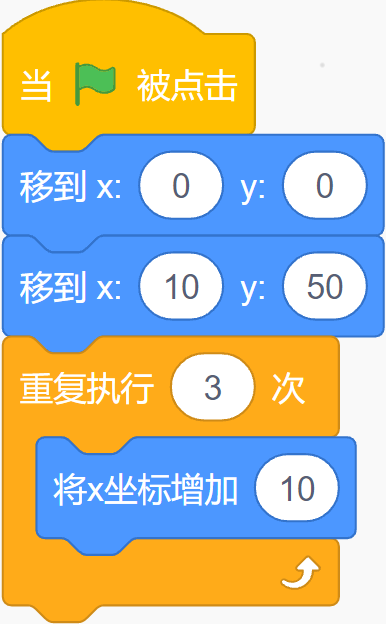
\includegraphics[width=\textwidth]{1.png}
                \caption*{第1题}
            \end{minipage}
            \begin{minipage}[t]{.35\textwidth}
                \centering
                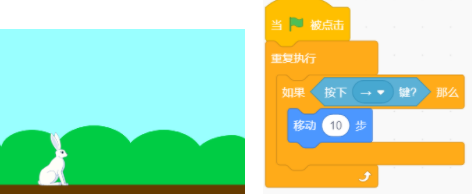
\includegraphics[width=\textwidth]{2.png}
                \caption*{第2题}
            \end{minipage}
            \begin{minipage}[t]{.12\textwidth}
                \centering
                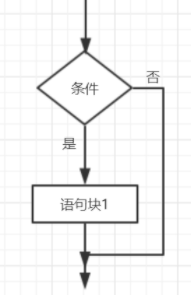
\includegraphics[width=\textwidth]{5.png}
                \caption*{第5题}
            \end{minipage}
            \begin{minipage}[t]{.35\textwidth}
                \centering
                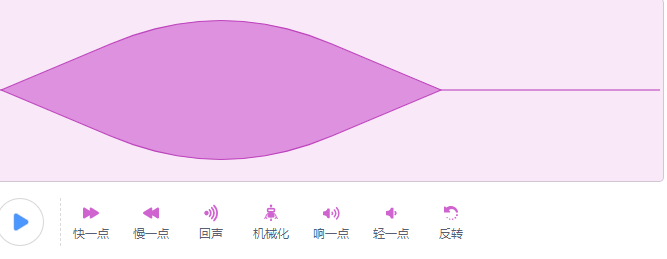
\includegraphics[width=\textwidth]{7.png}
                \caption*{第7题}
            \end{minipage}
        \end{figure}

        % 4
        \item 按照图中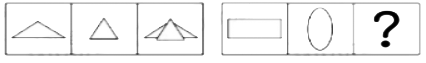
\includegraphics[width=.3\textwidth]{4.png}规则,在下列选项中找出所对应的图形?(\qquad)
        \begin{tasks}(4)
            \task 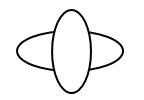
\includegraphics[width=.08\textwidth]{4a.png}
            \task 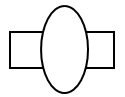
\includegraphics[width=.08\textwidth]{4b.png}
            \task 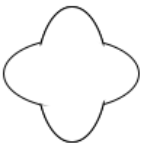
\includegraphics[width=.06\textwidth]{4c.png}
            \task 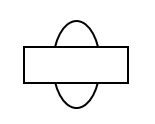
\includegraphics[width=.08\textwidth]{4d.png}
        \end{tasks}

        % 5
        \item 上面流程图可以用哪个积木实现?(\qquad)
        \begin{tasks}(4)
            \task 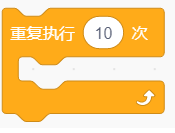
\includegraphics[width=.12\textwidth]{5a.png}
            \task 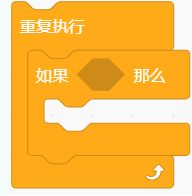
\includegraphics[width=.1\textwidth]{5b.png}
            \task 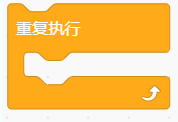
\includegraphics[width=.12\textwidth]{5c.png}
            \task 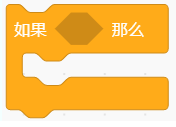
\includegraphics[width=.12\textwidth]{5d.png}
        \end{tasks}

        % 6
        \item 积木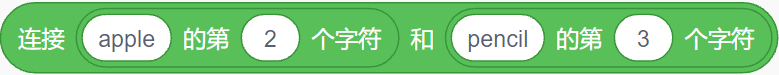
\includegraphics[width=.35\textwidth]{6.png}运行结果是?(\qquad)
        \begin{tasks}(4)
            \task pp
            \task ap
            \task np
            \task pn
        \end{tasks}

        % 7
        \item 上面哪个按钮,可以让声音变大一点儿?(\qquad)
        \begin{tasks}(4)
            \task 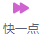
\includegraphics[width=.05\textwidth]{7a.png}
            \task 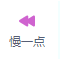
\includegraphics[width=.06\textwidth]{7b.png}
            \task 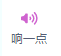
\includegraphics[width=.06\textwidth]{7c.png}
            \task 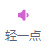
\includegraphics[width=.06\textwidth]{7d.png}
        \end{tasks}

        \newpage
       % 8
       \item 现在红绿灯的状态为绿灯,执行程序20秒后是什么灯亮?(\qquad)
       \begin{tasks}(4)
           \task 红灯亮
           \task 绿灯亮
           \task 红灯绿灯都不亮
           \task 红灯绿灯一起亮
       \end{tasks}

        % 9
        \item 当前篮球角色坐标为$(10,-110)$,篮筐坐标为$(10,130)$,执行程序后按下哪个键可以让篮球移动到篮筐中?(\qquad)
        \begin{tasks}(4)
            \task 按空格键
            \task 按$\uparrow$键
            \task 按$\downarrow$键
            \task 按任意键
        \end{tasks}

        \begin{figure}[htbp]
            \centering
            \begin{minipage}[t]{.28\textwidth}
                \centering
                \begin{minipage}[t]{.4\textwidth}
                    \centering
                    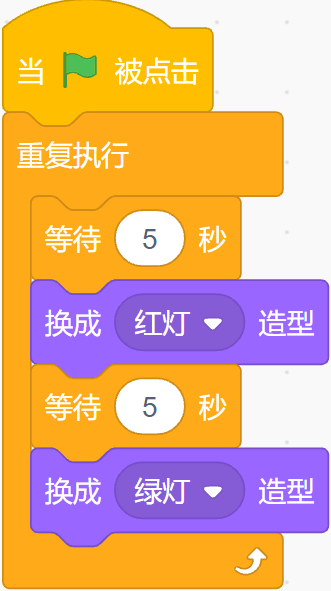
\includegraphics[width=\textwidth]{8-1.png}
                \end{minipage}
                \begin{minipage}[t]{.55\textwidth}
                    \centering
                    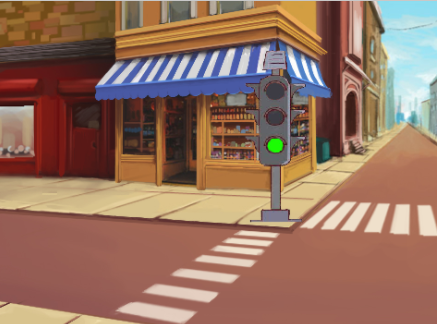
\includegraphics[width=\textwidth]{8-2.png}
                \end{minipage}
                \caption*{第8题}
            \end{minipage}
            \begin{minipage}[t]{.34\textwidth}
                \centering
                \begin{minipage}[t]{.58\textwidth}
                    \centering
                    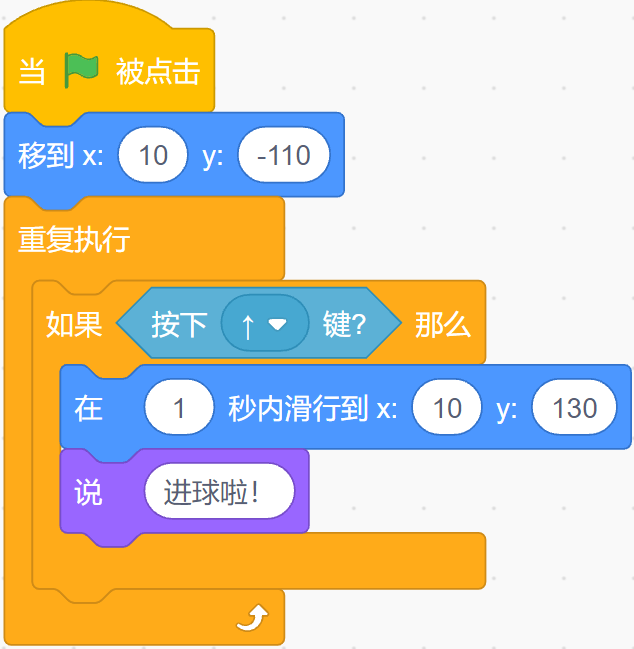
\includegraphics[width=\textwidth]{9-1.png}
                \end{minipage}
                \begin{minipage}[t]{.4\textwidth}
                    \centering
                    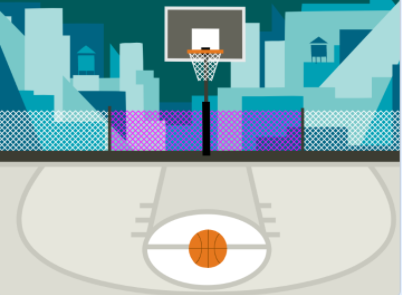
\includegraphics[width=\textwidth]{9-2.png}
                \end{minipage}
                \caption*{第9题}
            \end{minipage}
            \begin{minipage}[t]{.3\textwidth}
                \centering
                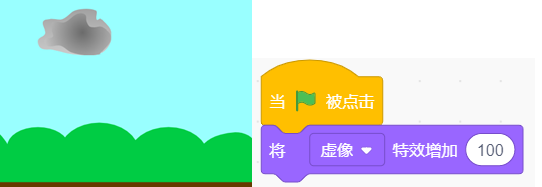
\includegraphics[width=\textwidth]{10.png}
                \caption*{第10题}
            \end{minipage}
        \end{figure}

        % 10
        \item 如上图,一朵乌云飘在空中,点击绿旗,乌云角色将有什么变化?(\qquad)
        \begin{tasks}(4)
            \task 乌云消失
            \task 乌云没有变化
            \task 乌云变多
            \task 乌云颜色变深了
        \end{tasks}

        % 11
        \item 如下图所示,积木
\includegraphics[width=.1\textwidth]{11-1.png}的颜色和红灯颜色一致,点击绿旗后,女该会?(\qquad)
        \begin{tasks}(4)
            \task 女孩说“红灯停”
            \task 移动10步
            \task 向左转弯
            \task 向右转弯
        \end{tasks}

        % 12
        \item 小猴和小兔去摘桃,小猴摘下15个桃,当小猴将自己的桃分3个给小兔子时,它俩的桃就一样多,小兔子摘了多少个桃?(\qquad)
        \begin{tasks}(4)
            \task 8
            \task 9
            \task 7
            \task 10
        \end{tasks}

        \begin{figure}[htbp]
            \centering
            \begin{minipage}[t]{.32\textwidth}
                \centering
                \begin{minipage}[t]{.48\textwidth}
                    \centering
                    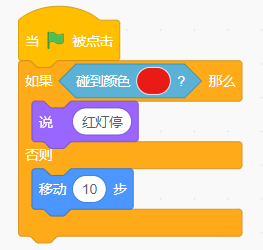
\includegraphics[width=\textwidth]{11-2.png}
                \end{minipage}
                \begin{minipage}[t]{.5\textwidth}
                    \centering
                    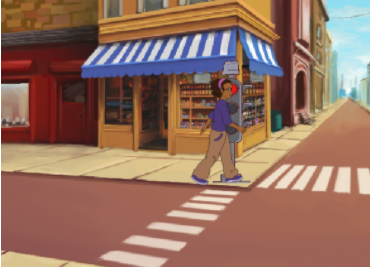
\includegraphics[width=\textwidth]{11-3.png}
                \end{minipage}
                \caption*{第11题}
            \end{minipage}
            \begin{minipage}[t]{.18\textwidth}
                \centering
                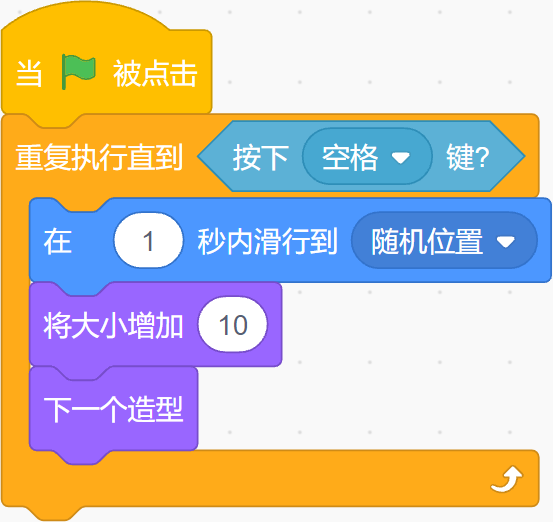
\includegraphics[width=\textwidth]{13.png}
                \caption*{第13题}
            \end{minipage}
            \begin{minipage}[t]{.45\textwidth}
                \centering
                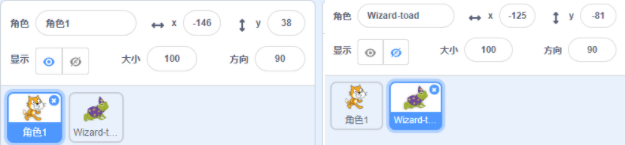
\includegraphics[width=\textwidth]{15.png}
                \caption*{第15题}
            \end{minipage}
        \end{figure}

        % 13
        \item 对于默认的小猫角色,执行上面程序,说法错误的是?(\qquad)
        \begin{tasks}(2)
            \task 不按下空格键,小猫会随机移动
            \task 不按下空格键,小猫会逐渐变大
            \task 不按下空格键,小猫会切换造型
            \task 当按下空格键,小猫一直移动
        \end{tasks}

        % 14
        \item 下面哪个积木运行结果是true?(\qquad)
        \begin{tasks}(4)
            \task 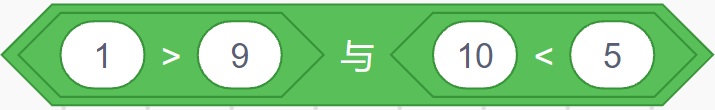
\includegraphics[width=.18\textwidth]{14a.png}
            \task 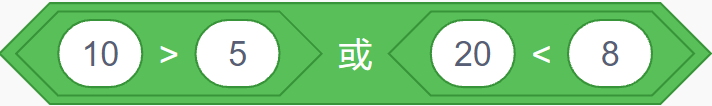
\includegraphics[width=.18\textwidth]{14b.png}
            \task 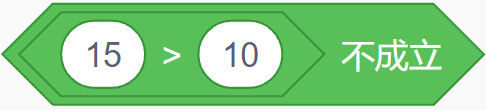
\includegraphics[width=.12\textwidth]{14c.png}
            \task 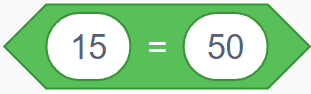
\includegraphics[width=.1\textwidth]{14d.png}
        \end{tasks}
        
        % 15
        \item 角色列表区如上图所示,舞台上角色显示正确的是?(\qquad)
        \begin{tasks}(4)
            \task 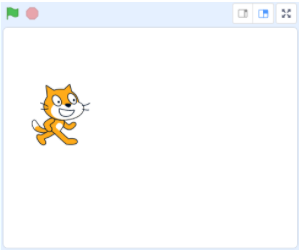
\includegraphics[width=.15\textwidth]{15a.png}
            \task 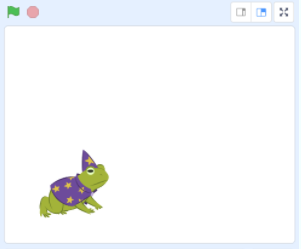
\includegraphics[width=.15\textwidth]{15b.png}
            \task 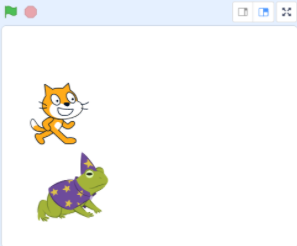
\includegraphics[width=.15\textwidth]{15c.png}
            \task 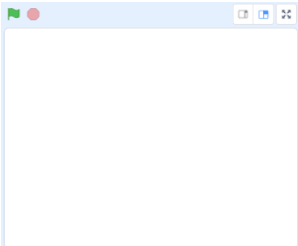
\includegraphics[width=.15\textwidth]{15d.png}
        \end{tasks}

        \newpage
        \item 按照图中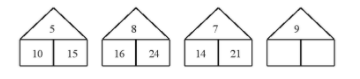
\includegraphics[width=.25\textwidth]{16.png}规则,第四个图形应该填入什么数写?(\qquad)
        \begin{tasks}(4)
            \task 左:18,右:27
            \task 左:10,右:15
            \task 左:27,右:27
            \task 左:9, 右:27
        \end{tasks}

        % 17
        \item 下面哪个程序可以将画笔的颜色设置为红色,画笔的粗细设置为10?(\qquad)
        \begin{tasks}(4)
            \task 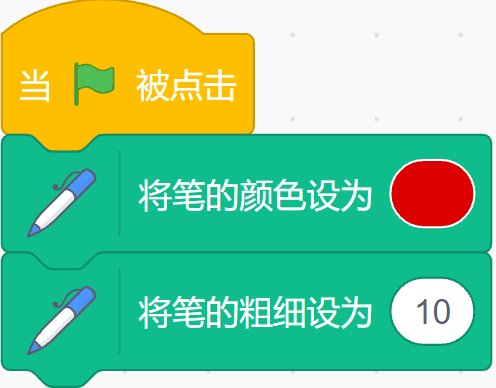
\includegraphics[width=.12\textwidth]{17a.png}
            \task 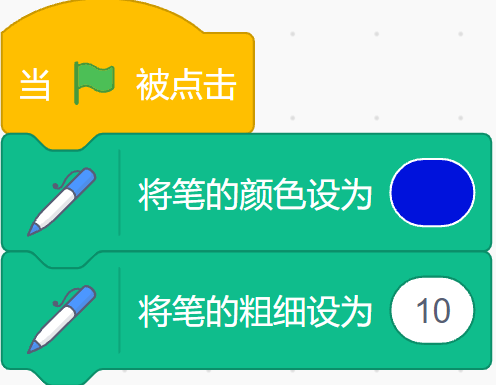
\includegraphics[width=.12\textwidth]{17b.png}
            \task 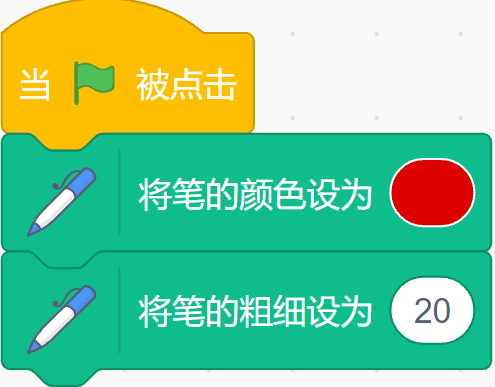
\includegraphics[width=.12\textwidth]{17c.png}
            \task 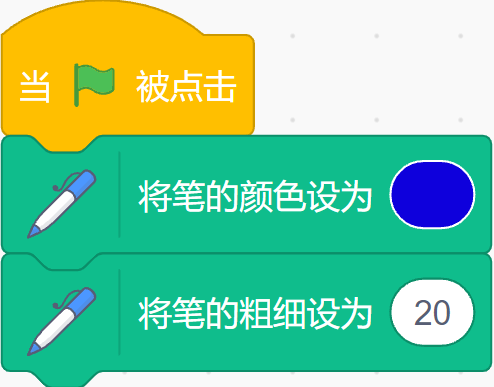
\includegraphics[width=.12\textwidth]{17d.png}
        \end{tasks}

        % 18
        \item 积木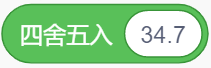
\includegraphics[width=.12\textwidth]{18.png}运行结果是?(\qquad)
        \begin{tasks}(4)
            \task 34
            \task 35
            \task 30
            \task 40
        \end{tasks}

        % 19
        \item 点击绿旗,鼠标碰到小象但是不按下鼠标键,小象角色会发生什么变化?(\qquad)
        \begin{tasks}(4)
            \task 小象没变化
            \task 换成elephant-b造型
            \task 小象消失了
            \task 换成elephant-b背景
        \end{tasks}

        % 20
        \item 执行下面程序,字母B将会有什么变?(\qquad)
        \begin{tasks}(4)
            \task 字母B变换颜色闪烁
            \task 字母B最后消失不见
            \task 字母B只剩轮廓
            \task 字母B没有变化
        \end{tasks}

        % 21
        \item 气球当前大小为40,只点击一次绿旗,气球角色的大小将变为多少?(\qquad)
        \begin{tasks}(4)
            \task 50
            \task 60
            \task 70
            \task 80
        \end{tasks}

        \begin{figure}[htbp]
            \centering
            \begin{minipage}[t]{.36\textwidth}
                \centering
                \begin{minipage}[t]{.4\textwidth}
                    \centering
                    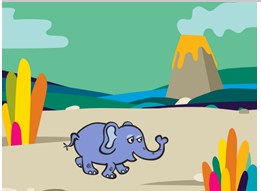
\includegraphics[width=\textwidth]{19-1.png}
                \end{minipage}
                \begin{minipage}[t]{.58\textwidth}
                    \centering
                    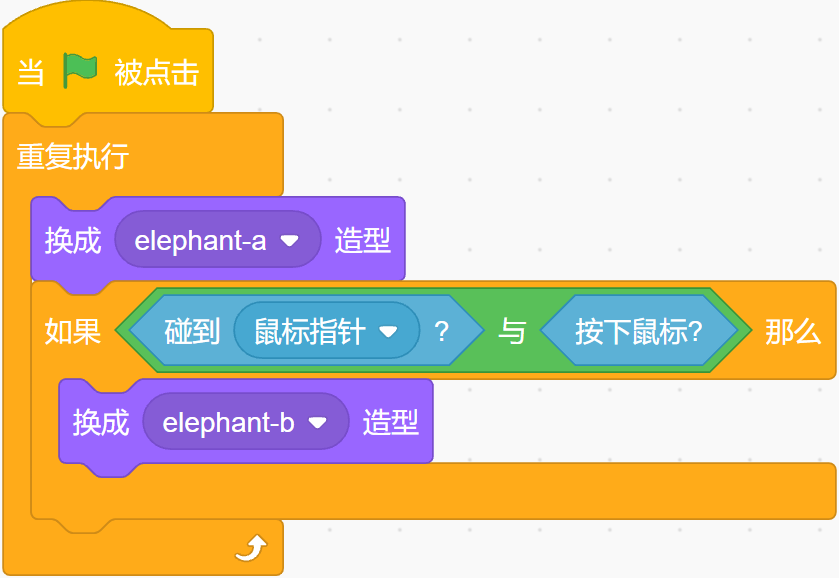
\includegraphics[width=\textwidth]{19-2.png}
                \end{minipage}
                \caption*{第19题}
            \end{minipage}
            \begin{minipage}[t]{.32\textwidth}
                \centering
                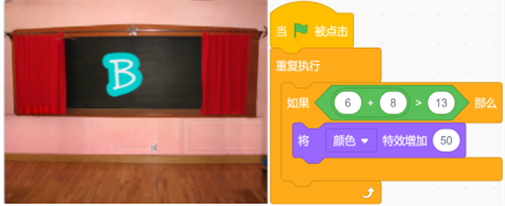
\includegraphics[width=\textwidth]{20.png}
                \caption*{第20题}
            \end{minipage}
            \begin{minipage}[t]{.3\textwidth}
                \centering
                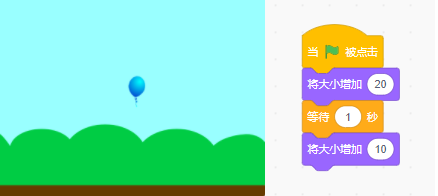
\includegraphics[width=\textwidth]{21.png}
                \caption*{第21题}
            \end{minipage}
        \end{figure}

        % 22
        \item 蜻蜓正在天空飞行,积木的颜色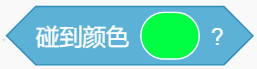
\includegraphics[width=.1\textwidth]{22-1.png}和绿树的颜色是一样的,运行以下哪个程序可以让蜻蜓飞到绿树上,并且停止飞行?(\qquad)
        \begin{figure}[htbp]
            \begin{minipage}{.2\textwidth}
                \centering
                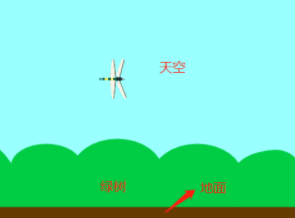
\includegraphics[width=\textwidth]{22-2.png}
            \end{minipage}
            \begin{minipage}{.78\textwidth}
                \begin{tasks}(4)
                    \task 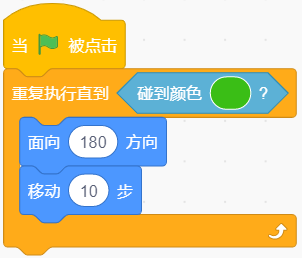
\includegraphics[width=.18\textwidth]{22a.png}
                    \task 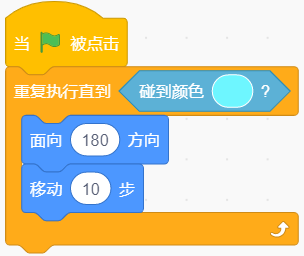
\includegraphics[width=.18\textwidth]{22b.png}
                    \task \includegraphics[width=.12\textwidth]{22c.png}
                    \task \includegraphics[width=.12\textwidth]{22d.png}
                \end{tasks}
            \end{minipage}
        \end{figure}

        % 23
        \item 下面流程图可以用哪个积木实现?(\qquad)
        
        \begin{minipage}{.11\textwidth}
            \centering
            \includegraphics[width=\textwidth]{23.png}
        \end{minipage}
        \begin{minipage}{.78\textwidth}
            \begin{tasks}(4)
                \task \includegraphics[width=.18\textwidth]{23a.png}
                \task \includegraphics[width=.18\textwidth]{23b.png}
                \task \includegraphics[width=.18\textwidth]{23c.png}
                \task \includegraphics[width=.12\textwidth]{23d.png}
            \end{tasks}
        \end{minipage}

        \newpage
        % 24
        \item 下面程序中“?”处填写哪个数字可以让角色发出喵的声音?(\qquad)
        \begin{tasks}(4)
            \task 44
            \task 15
            \task 88
            \task 23
        \end{tasks}

        % 25
        \item 下面程序会绘制出什么图形?(\qquad)
        \begin{tasks}(4)
            \task 三角形
            \task 圆形
            \task 正方形
            \task 五角星
        \end{tasks}
    \end{enumerate}

    \begin{figure}[htbp]
        \centering
        \begin{minipage}[t]{.16\textwidth}
            \centering
            \includegraphics[width=\textwidth]{24.png}
            \caption*{第24题}
        \end{minipage}
        \begin{minipage}[t]{.15\textwidth}
            \centering
            \includegraphics[width=\textwidth]{25.png}
            \caption*{第25题}
        \end{minipage}
        \begin{minipage}[t]{.14\textwidth}
            \centering
            \includegraphics[width=\textwidth]{26.png}
            \caption*{第26题}
        \end{minipage}
        \begin{minipage}[t]{.2\textwidth}
            \centering
            \includegraphics[width=\textwidth]{27.png}
            \caption*{第27题}
        \end{minipage}
        \begin{minipage}[t]{.16\textwidth}
            \centering
            \includegraphics[width=\textwidth]{28.png}
            \caption*{第28题}
        \end{minipage}
    \end{figure}

    % 判断题
    {\noindent\textbf{第二部分、判断题(共 10 题,每题 2 分,共20分.)}}
    \begin{enumerate}
        \setcounter{enumi}{25}
        % 26
        \item 如上图,点击绿旗,小狗角色只播放声音“汪”5次,不做其他操作.(\qquad)

        %27
        \item 流星当前坐标为(120,100),执行上面程序,流星滑行到坐标为($-200,0$)的位置.(\qquad)
        
        %28
        \item 怪物的位置和程序如上图所示,积木中的颜色和气球颜色一致,点击绿旗,怪物角色会换成frank-a造型.(\qquad)

        %29
        \item 执行程序\includegraphics[width=.3\textwidth]{29.png},只按下a键,角色就能移动50步.(\qquad)
        
        \begin{figure}[htbp]
            \centering
            \begin{minipage}[t]{.16\textwidth}
                \centering
                \includegraphics[width=\textwidth]{30.png}
                \caption*{第30题}
            \end{minipage}
            \begin{minipage}[t]{.18\textwidth}
                \centering
                \includegraphics[width=\textwidth]{31.png}
                \caption*{第31题}
            \end{minipage}
            \begin{minipage}[t]{.4\textwidth}
                \centering
                \includegraphics[width=\textwidth]{32.png}
                \caption*{第32题}
            \end{minipage}
            \begin{minipage}[t]{.1\textwidth}
                \centering
                \includegraphics[width=\textwidth]{33.png}
                \caption*{第33题}
            \end{minipage}
            \begin{minipage}[t]{.12\textwidth}
                \centering
                \includegraphics[width=\textwidth]{35.png}
                \caption*{第35题}
            \end{minipage}
        \end{figure}
        
        %30
        \item 如上图,点击绿旗,鼠标碰到蝴蝶后,蝴蝶滑行到随机位置.(\qquad)
        
        %31
        \item 立方体的每个面上都有一个数字,其平面展开如上图所示。在这个立方体中,“\ding{176}”对面的数字是“\ding{172}”.(\qquad)
        
        %32
        \item 上图两组程序实现的效果一样:小猫碰到鼠标停止,只要不碰到鼠标就一直跟着鼠标移动.(\qquad)
        
        %33
        \item 执行上面程序音量变小了.(\qquad)
        
        %34
        \item 积木\includegraphics[width=.3\textwidth]{34.png}运行结果为true.(\qquad)
        
        %35
        \item 上面程序可以绘制出一条红色直线.(\qquad)
    \end{enumerate}

    \newpage
    {\noindent \textbf{第三部分、编程题(共 2 题,共30分.)}}
    \begin{enumerate}
        \setcounter{enumi}{35}
        
        % 36
        \item 森林聚会1:
        \begin{figure}[htbp]
            \begin{minipage}{.6\textwidth}
                1. 准备工作
                \begin{tasks}[label = (\arabic*)]
                    \task 导入背景Jungle;
                    \task 角色Dragon、Fairy、Hippo1、Grifin、Wizard.
                \end{tasks}
                2. 功能实现
                \begin{tasks}[label = (\arabic*)]
                    \task 点击绿旗,角色的初始位置和方向如图所示;
                    \task 等待1秒,魔法师和小动物们调整方向,不断移动,碰到边缘就反弹;
                    \task 用上、下、左、右键,小精灵水平垂直飞行,不需要调整面向方向;
                    魔法师碰到小精灵,魔法师将会消失,停止全部脚本;
                    \task 小动物碰到魔法师,小动物说“救命!”0.5秒后消失,表示动物已被抓走.
                \end{tasks}
            \end{minipage}
            \begin{minipage}{.37\textwidth}
                \centering
                \includegraphics[width=\textwidth]{36.png}
            \end{minipage}
        \end{figure}

        %37
        \item 绘制图形:
        \begin{figure}[htbp]
            \begin{minipage}{.6\textwidth}
                1. 准备工作
                \begin{tasks}[label = (\arabic*)]
                    \task 保留默认小猫角色,隐藏角色;
                    \task 背景为默认白色背景.
                \end{tasks}
                2. 功能实现
                \begin{tasks}[label = (\arabic*)]
                    \task 小猫的初始位置为($x:0,y:0$)
                    \task 线条粗细为3,颜色为红色,正方形的边长为50,每个正方形之间相隔25;
                    \task 画出所示图形.
                \end{tasks}
            \end{minipage}
            \begin{minipage}{.37\textwidth}
                \centering
                \includegraphics[width=.6\textwidth]{37.png}
            \end{minipage}
        \end{figure}
    \end{enumerate}
\end{document}